\documentclass[12pt,a4paper]{article}

% ─── Packages ────────────────────────────────────────────────────────────────
\usepackage[margin=2.5cm, headheight=25pt]{geometry}
\usepackage{xcolor}
\usepackage{fontenc}
\usepackage{inputenc}
\usepackage{lmodern}
\usepackage[explicit]{titlesec}
\usepackage{booktabs}
\usepackage{tabularx}
\usepackage{array}
\usepackage{colortbl}
\usepackage{graphicx}
\usepackage{tikz}
\usepackage{tikz-cd}
\usepackage{mdframed}
\usepackage{enumitem}
\usepackage{fancyhdr}
\usepackage{hyperref}
\usepackage{listings}
\usepackage{tcolorbox}
\usepackage{multicol}
\usepackage{makecell}
\usepackage{float}
\usepackage{amsmath}

\usetikzlibrary{shapes.geometric, arrows.meta, positioning, fit, backgrounds, shadows}

% ─── Colour Palette ──────────────────────────────────────────────────────────
\definecolor{NavyBlue}{HTML}{1A2B4A}
\definecolor{OceanBlue}{HTML}{1B6CA8}
\definecolor{TealAccent}{HTML}{0D9B8A}
\definecolor{WaveGreen}{HTML}{2ECC71}
\definecolor{CoralRed}{HTML}{E74C3C}
\definecolor{SunGold}{HTML}{F39C12}
\definecolor{LightGray}{HTML}{F4F6F9}
\definecolor{MidGray}{HTML}{BDC3C7}
\definecolor{DarkGray}{HTML}{2C3E50}
\definecolor{PurpleAccent}{HTML}{8E44AD}
\definecolor{CodeBg}{HTML}{1E2832}
\definecolor{BossRed}{HTML}{C0392B}

% ─── Hyperref Setup ──────────────────────────────────────────────────────────
\hypersetup{colorlinks=true, linkcolor=OceanBlue, urlcolor=TealAccent}

% ─── Section Title Styling ───────────────────────────────────────────────────
\titleformat{\section}
  {\color{NavyBlue}\Large\bfseries}
  {}
  {0em}
  {\colorbox{NavyBlue}{\parbox{\dimexpr\linewidth-2\fboxsep}{\textcolor{white}{\thesection\quad #1}}}}

\titleformat{\subsection}
  {\color{OceanBlue}\large\bfseries}
  {\thesubsection}
  {0.5em}
  {#1}[\titlerule]

\titleformat{\subsubsection}
  {\color{TealAccent}\normalsize\bfseries}
  {\thesubsubsection}
  {0.5em}
  {#1}

% ─── Header / Footer ─────────────────────────────────────────────────────────
\pagestyle{fancy}
\fancyhf{}
\fancyhead[L]{\small\textcolor{OceanBlue}{\textbf{Phase 2 — One Piece: Raft Survivor}}}
\fancyhead[R]{\small\textcolor{MidGray}{Computer Graphics Project}}
\fancyfoot[C]{\small\textcolor{MidGray}{\thepage}}
\renewcommand{\headrulewidth}{0.4pt}
\renewcommand{\headrule}{\hbox to\headwidth{\color{OceanBlue}\leaders\hrule height \headrulewidth\hfill}}

% ─── Code Listing Style ──────────────────────────────────────────────────────
\lstdefinestyle{cppstyle}{
  backgroundcolor=\color{CodeBg},
  basicstyle=\ttfamily\small\color{white},
  keywordstyle=\color{cyan}\bfseries,
  commentstyle=\color{MidGray}\itshape,
  stringstyle=\color{WaveGreen},
  breaklines=true,
  frame=single,
  framerule=0.5pt,
  rulecolor=\color{OceanBlue},
  numbers=left,
  numberstyle=\tiny\color{MidGray},
  language=C++,
}

% ─── Coloured Boxes ──────────────────────────────────────────────────────────
\tcbuselibrary{skins, breakable}

\newtcolorbox{phasebox}[2][]{
  enhanced, breakable,
  title=#2,
  colback=LightGray, colframe=OceanBlue,
  fonttitle=\bfseries\color{white},
  attach boxed title to top left={yshift=-2mm, xshift=4mm},
  boxed title style={colback=OceanBlue, rounded corners},
  #1
}

\newtcolorbox{warningbox}{
  enhanced,
  colback=yellow!10, colframe=SunGold,
  leftrule=4pt,
  sharp corners=west,
}

\newtcolorbox{tipbox}{
  enhanced,
  colback=TealAccent!8, colframe=TealAccent,
  leftrule=4pt,
  sharp corners=west,
}

\newtcolorbox{fileref}{
  enhanced,
  colback=CodeBg!90!white, colframe=OceanBlue,
  fontupper=\ttfamily\small\color{white},
  sharp corners,
  left=6pt, right=6pt,
}

% ─── Document ─────────────────────────────────────────────────────────────────
\begin{document}

% ══════════════════════════════════════════════════════
%  TITLE PAGE
% ══════════════════════════════════════════════════════
\begin{titlepage}
\pagecolor{NavyBlue}
\color{white}
\vspace*{2cm}

\begin{center}

% Decorative wave line

\begin{tikzpicture}
  \draw[OceanBlue!60, line width=2pt, domain=0:14, samples=200]
    plot (\x, {0.2*sin(3*\x r)});
\end{tikzpicture}

\vspace{0.5cm}
{\fontsize{36}{44}\selectfont\bfseries One Piece: Raft Survivor}\\[0.3cm]
{\fontsize{18}{26}\selectfont\color{TealAccent} Phase 2 — Technical Design Document}\\[0.5cm]


\begin{tikzpicture}
  \draw[OceanBlue!60, line width=2pt, domain=0:14, samples=200]
    plot (\x, {0.2*sin(3*\x r + 3.14)});
\end{tikzpicture}

\vspace{1.5cm}

% Team Table on title page
\begin{tabular}{ccc}
\toprule
\textbf{Member} & \textbf{Name} & \textbf{Task Ownership (Vertical Slices)}\\
\midrule
Member 1 & \textit{(Team Member 1)} & Task 1: Foundations \& The Ocean\\
Member 2 & \textit{Mohamed} & Task 2: Survival \& Crafting\\
Member 3 & \textit{Ahmed Gamal} & Task 3: Ocean Predators (Sharks \& Marines)\\
Member 4 & \textit{Yousef} & Task 4: Epic Encounters (Kraken \& Penguin)\\
\bottomrule
\end{tabular}

\vspace{2cm}

{\large\color{MidGray} Computer Graphics · Due: 27 April 2026}

\vspace{1cm}

% Raft icon drawn in TikZ
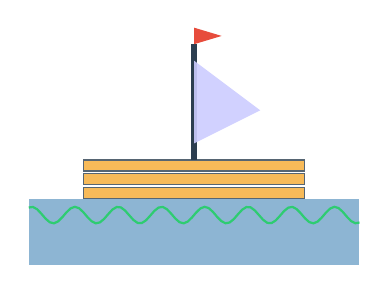
\begin{tikzpicture}[scale=0.7]
  % Water
  \fill[OceanBlue!50] (-3,-1.2) rectangle (3,0);
  \draw[WaveGreen, thick, domain=-3:3, samples=80]
    plot (\x, {-0.3 + 0.15*sin(8*\x r + 1)});
  % Raft planks
  \foreach \y in {0, 0.25, 0.5}{
    \fill[SunGold!70] (-2, \y) rectangle (2, \y+0.2);
    \draw[DarkGray!80, thin] (-2, \y) rectangle (2, \y+0.2);
  }
  % Mast
  \draw[DarkGray, line width=2pt] (0,0.7) -- (0, 2.8);
  % Sail
  \fill[white!80!blue, opacity=0.9]
    (0,1.0) -- (1.2,1.6) -- (0,2.5) -- cycle;
  % Flag
  \fill[CoralRed] (0,2.8) -- (0.5,2.95) -- (0,3.1) -- cycle;
\end{tikzpicture}

\end{center}
\vfill
\end{titlepage}
\pagecolor{white}\color{black}

% ══════════════════════════════════════════════════════
%  TABLE OF CONTENTS
% ══════════════════════════════════════════════════════
\tableofcontents
\newpage

% ══════════════════════════════════════════════════════
%  1. PROJECT OVERVIEW
% ══════════════════════════════════════════════════════
\section{Project Overview}

This document outlines the complete technical plan for \textbf{Phase 2} of the One Piece: Raft Survivor game, built on a custom C++ OpenGL Engine using an Entity Component System (ECS). 
Phase 2 shifts toward a full implementation of the game loop: interacting with the sea environment, fighting oceanic beasts and marines, progressing through waves of enemies, and finally meeting a giant penguin to win the "One Piece".

\vspace{1em}
To ensure all members get hands-on experience with both \textbf{Graphics/Shaders (OpenGL)} and \textbf{Core Logic (C++)}, work is divided into \textbf{Vertical Slices}. This means each member owns a specific feature from the mathematical shader rendering up to the gameplay loops.
\vspace{1em}

\begin{center}
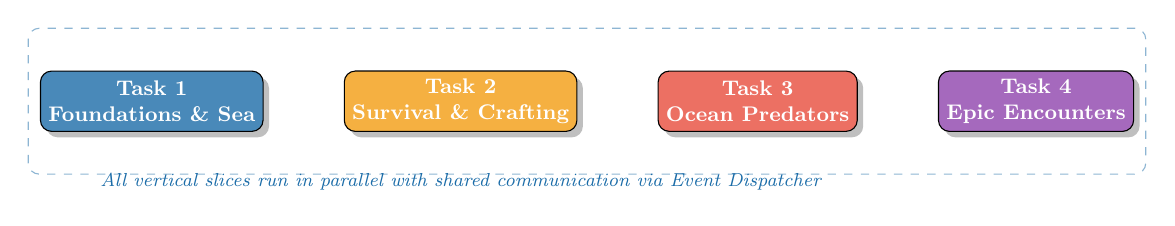
\begin{tikzpicture}[scale=0.85, transform shape,
  node distance=1.6cm and 1.2cm,
  box/.style={draw, rounded corners=4pt, minimum width=2.6cm, minimum height=0.9cm,
              align=center, font=\small\bfseries, drop shadow},
  arrow/.style={-{Stealth[length=6pt]}, thick}
]
  \node[box, fill=OceanBlue!80, text=white] (T1) {Task 1\\Foundations \& Sea};
  \node[box, fill=SunGold!80, text=white, right=of T1] (T2) {Task 2\\Survival \& Crafting};
  \node[box, fill=CoralRed!80, text=white, right=of T2] (T3) {Task 3\\Ocean Predators};
  \node[box, fill=PurpleAccent!80, text=white, right=of T3] (T4) {Task 4\\Epic Encounters};

  % Parallel work annotation
  \draw[dashed, OceanBlue!50, rounded corners]
    ([xshift=-5pt,yshift=-18pt]T1.south west) rectangle ([xshift=5pt,yshift=18pt]T4.north east);
  \node[below=0.5cm of T2, font=\footnotesize\itshape, text=OceanBlue]
    {All vertical slices run in parallel with shared communication via Event Dispatcher};
\end{tikzpicture}
\end{center}

% ══════════════════════════════════════════════════════
%  2. GAME FLOW DIAGRAM
% ══════════════════════════════════════════════════════
\section{Game Flow \& Wave State Machine}

The game flow is separated into chronological sequences that challenge the player's resource management and combat skills.

\vspace{1em}
\begin{center}
\resizebox{\textwidth}{!}{
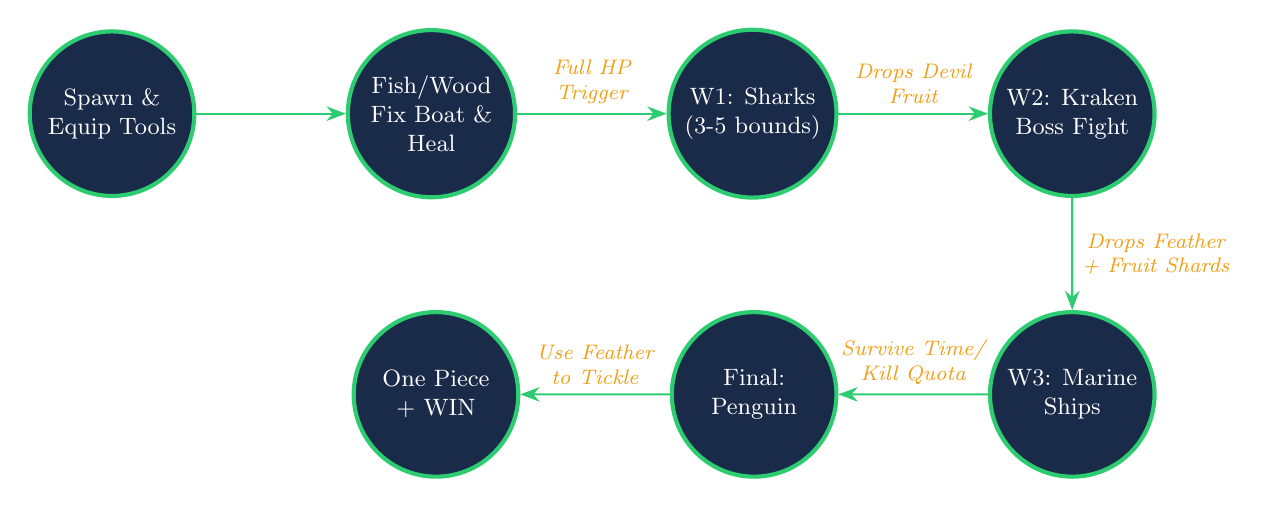
\begin{tikzpicture}[scale=0.95, transform shape,
  node distance=1.3cm and 2cm,
  circle_node/.style={circle, draw=WaveGreen, line width=1.5pt,
    fill=NavyBlue, text=white, align=center, minimum size=2.2cm, font=\small},
  arrow/.style={-{Stealth[length=7pt]}, WaveGreen, thick},
  label_style/.style={font=\footnotesize\itshape, text=SunGold, align=center}
]

  \node[circle_node] (start) {Spawn \&\\Equip Tools};
  \node[circle_node, right=2cm of start] (recovery) {Fish/Wood\\Fix Boat \&\\Heal};
  \node[circle_node, right=2cm of recovery] (sharks) {W1: Sharks\\(3-5 bounds)};
  \node[circle_node, right=2cm of sharks] (kraken) {W2: Kraken\\Boss Fight};
  
  \node[circle_node, below=1.5cm of kraken] (marines) {W3: Marine\\Ships};
  \node[circle_node, left=2cm of marines] (penguin) {Final:\\Penguin};
  \node[circle_node, left=2cm of penguin] (win) {One Piece\\+ WIN};

  \draw[arrow] (start) -- (recovery);
  \draw[arrow] (recovery) -- node[above, label_style]{Full HP\\Trigger} (sharks);
  \draw[arrow] (sharks) -- node[above, label_style]{Drops Devil\\Fruit} (kraken);
  \draw[arrow] (kraken) -- node[right, label_style]{Drops Feather\\+ Fruit Shards} (marines);
  \draw[arrow] (marines) -- node[above, label_style]{Survive Time/\\Kill Quota} (penguin);
  \draw[arrow] (penguin) -- node[above, label_style]{Use Feather\\to Tickle} (win);

\end{tikzpicture}
}
\end{center}

% ══════════════════════════════════════════════════════
%  3. TASK 1 — FOUNDATIONS & THE OCEAN
% ══════════════════════════════════════════════════════
\section{Task 1 — Foundations \& The Ocean}

\subsection{Overview}
Build the core environment, moving sea elements, and basic player controls.

\begin{itemize}[leftmargin=*]
    \item \textbf{Graphics (OpenGL):} 
    \begin{itemize}
        \item \textbf{Sea Shader:} Implement Gerstner Waves math in \texttt{water.vert} to create rolling, peaked waves so that the water is not just a flat plane.
        \item \textbf{Skybox/Lighting:} Setup a cubemap for the clear sky and sun as the main light source. Integrate basic Phong or PBR lighting so the scene casts proper shadows/lighting on the raft.
    \end{itemize}
    \item \textbf{Logic (C++):}
    \begin{itemize}
        \item \textbf{Input \& Movement:} Map WASD, Space for jumps, and Motion Camera. 
        \item \textbf{Buoyancy Math:} Replicate the Gerstner wave calculations in C++ to compute the exact $(x,z)$ height. Ensure the boat and player "bob" on the waves rather than clipping through them.
    \end{itemize}
\end{itemize}

% ══════════════════════════════════════════════════════
%  4. TASK 2 — SURVIVAL & CRAFTING
% ══════════════════════════════════════════════════════
\section{Task 2 — Survival \& Crafting (The Raft Core)}

\subsection{Overview}
Manage the player's core gameplay loop of staying alive, collecting resources, and UI overlays.

\begin{itemize}[leftmargin=*]
    \item \textbf{Graphics (OpenGL):}
    \begin{itemize}
        \item \textbf{HUD Rendering:} Draw 2D overlays using Orthographic projection. Position the Health bar (bottom left), Devil Fruit power bar (above health), and Inventory selection (bottom).
        \item \textbf{Mesh/Textures Strategy:} Load missing chunk models. When a part of the boat is destroyed, swap the visible plank mesh so it visually breaks down.
    \end{itemize}
    \item \textbf{Logic (C++):}
    \begin{itemize}
        \item \textbf{Inventory System:} Store items (Hammer, Spear, Net/Fishing rod). Map keys 1, 2, 3, 4 to equip tools respectively. Handle fishing states.
        \item \textbf{Health/Repair System:} Logic for eating fish (restores Player HP) and fixing the boat using wood (restores Ship HP and re-enables missing mesh chunks).
    \end{itemize}
\end{itemize}

% ══════════════════════════════════════════════════════
%  5. TASK 3 — OCEAN PREDATORS (SHARKS & MARINES)
% ══════════════════════════════════════════════════════
\section{Task 3 — Ocean Predators (Sharks \& Marines)}

\subsection{Overview}
Spawn enemies, calculate AI movements, and handle incoming damage and ship projectiles.

\begin{itemize}[leftmargin=*]
    \item \textbf{Graphics (OpenGL):}
    \begin{itemize}
        \item \textbf{Model Management:} Use Assimp to load Shark and Marine Ship templates. 
        \item \textbf{Damage Visuals:} Shader effect for hit indicators (e.g., flash red when players strike a shark). Render cannonballs and bullets flying through the air.
    \end{itemize}
    \item \textbf{Logic (C++):}
    \begin{itemize}
        \item \textbf{Shark AI:} 3-5 Sharks that circle the boat, approach into melee range, and deplete ship HP. Calculate player spear intersections using Raycasting. Disburse a Devil Fruit drop on full wave completion.
        \item \textbf{Marine AI:} Implement 2 ship sizes. Manage ships firing cannons and bullets (projectiles) toward the player's location. Keep an internal timer/counter for the invasion retreat condition.
    \end{itemize}
\end{itemize}

% ══════════════════════════════════════════════════════
%  6. TASK 4 — EPIC ENCOUNTERS (KRAKEN & PENGUIN)
% ══════════════════════════════════════════════════════
\section{Task 4 — Epic Encounters (Kraken \& Penguin)}

\subsection{Overview}
Develop complex boss attack phases, animations, large UI elements, and the win condition sequence.

\begin{itemize}[leftmargin=*]
    \item \textbf{Graphics (OpenGL):}
    \begin{itemize}
        \item \textbf{Boss Animations:} Drive the Kraken tentacles using hierarchical transforms or Inverse Kinematics (IK). Visually telegraph when an attack is about to swing.
        \item \textbf{Boss UI:} Implement the giant boss health bar at the top of the screen. 
    \end{itemize}
    \item \textbf{Logic (C++):}
    \begin{itemize}
        \item \textbf{Kraken State Machine:} Wait $\rightarrow$ Windup (Vulnerable) $\rightarrow$ Swing (Damages Player and Ship). Drop Giant Feather + Fruit shards on death.
        \item \textbf{Penguin \& Win Condition:} Create the giant sad penguin interaction. Detect if the player currently has the Giant Feather equipped to "tickle" it, triggering the happiness state and final Win screen sequence.
    \end{itemize}
\end{itemize}

% ══════════════════════════════════════════════════════
%  7. EVENT-DRIVEN ARCHITECTURE EXPLAINED
% ══════════════════════════════════════════════════════
\section{Event-Driven Architecture (Implementation Tip)}

To ensure these tasks operate seamlessly without tightly coupling the codebase (i.e. to avoid a giant "if-else" mess), Phase 2 will heavily utilize an \textbf{Event Dispatcher Pattern}.

\begin{lstlisting}[style=cppstyle, caption={Event Dispatcher Example}]
// 1. Define typical game events
enum class GameEvent { PLAYER_HIT, SHARK_DEATH, BOAT_DAMAGED };

// 2. Systems can "fire" events decoupled from the receivers
void SharkSystem::Update() {
    if (sharkBitesBoat) {
        EventDispatcher::Trigger(GameEvent::BOAT_DAMAGED, damageAmount);
    }
}

// 3. Other systems listen and react asynchronously
void HudSystem::OnNotify(GameEvent event, int value) {
    if (event == GameEvent::BOAT_DAMAGED) {
        FlashScreenRed();
        LowerShipHealth(value);
    }
}
\end{lstlisting}

% ══════════════════════════════════════════════════════
%  8. ASSETS & LIBRARIES
% ══════════════════════════════════════════════════════
\section{Assets \& Libraries Guide}

\begin{tcolorbox}[
  enhanced, colback=CodeBg!90!white, colframe=NavyBlue,
  fontupper=\small\color{white}, sharp corners, left=8pt, right=8pt]
\textbf{3D Models (.obj, .fbx):}
\begin{itemize}
    \item \textbf{Sketchfab} \& \textbf{Poly.pizza:} High quality and low-poly assets with Creative Commons licensing. Perfect for generic "One Piece" looking characters, rafts, and tools.
    \item \textbf{Mixamo (by Adobe):} For humanoid player models. You can upload a standard T-pose model and download walking/running/attack animations.
    \item \textbf{The Models Resource:} Ripped assets from old games. Good for placeholders.
\end{itemize}

\textbf{Textures \& Skies:}
\begin{itemize}
    \item \textbf{Poly Haven:} Best for high-quality PBR textures (Wood planks) and HDRIs for Skyboxes.
\end{itemize}

\textbf{C++ Libraries to Utilize:}
\begin{itemize}
    \item \textbf{Assimp:} Crucial for loading `.obj` or `.fbx` models into the OpenGL runtime.
    \item \textbf{GLM:} Essential for executing Matrix algorithms, cross products, and camera setup.
    \item \textbf{STB\_Image:} Single-header library ideal for texture loading.
\end{itemize}
\end{tcolorbox}

% ══════════════════════════════════════════════════════
%  9. PDF REPORT REQUIREMENTS
% ══════════════════════════════════════════════════════
\section{PDF Report Requirements}

\begin{warningbox}
\textbf{Phase 2 PDF Report due: 27 April 2026}
\end{warningbox}

\begin{enumerate}[leftmargin=*, itemsep=4pt]
  \item Team member names and IDs
  \item Contribution breakdown per member (map each feature to a name based on the Vertical Slice owned)
  \item At least \textbf{3 screenshots} from the running game showcasing Bosses, shaders, and UI.
\end{enumerate}

\vspace{1em}
\begin{center}

\begin{tikzpicture}
  \draw[NavyBlue, line width=1pt, domain=0:14, samples=200]
    plot (\x, {0.15*sin(4*\x r)});
\end{tikzpicture}

\vspace{0.4em}
\textit{\textcolor{MidGray}{End of Phase 2 Technical Design Document}}
\end{center}

\end{document}n